\documentclass[conference]{IEEEtran}
\IEEEoverridecommandlockouts

\usepackage{cite}
\usepackage{amsmath,amssymb,amsfonts}
\usepackage{graphicx}
\usepackage{textcomp}
\usepackage{xcolor}
\usepackage{booktabs}

\def\BibTeX{{\rm B\kern-.05em{\sc i\kern-.025em b}\kern-.08em
    T\kern-.1667em\lower.7ex\hbox{E}\kern-.125emX}}

\begin{document}

\title{Reproducing the Apparent Quantum-Kernel Advantage of Rydberg-Atom DAQCNN using Classical Nonlinearity}

\author{\IEEEauthorblockN{Anonymous Authors}}

\maketitle

% compact vertical spacing (whitespace only, no content change)
\setlength{\textfloatsep}{6pt plus 2pt minus 2pt}
\setlength{\dbltextfloatsep}{7pt plus 2pt minus 2pt}
\setlength{\floatsep}{6pt plus 2pt minus 2pt}
\setlength{\intextsep}{6pt plus 2pt minus 2pt}
\setlength{\abovedisplayskip}{3pt plus 1pt minus 1pt}
\setlength{\belowdisplayskip}{3pt plus 1pt minus 1pt}
\setlength{\abovedisplayshortskip}{1pt plus 1pt}
\setlength{\belowdisplayshortskip}{2pt plus 1pt minus 1pt}

\begin{abstract}
We test whether the quantum-kernel advantage reported for digital-analog
quantum convolutional neural networks (DAQCNN) with neutral-atom Rydberg kernels
reflects quantum structure or is an artifact of classifier capacity and feature
nonlinearity. Using a van der Waals Rydberg Hamiltonian, we disentangle three
design choices, the encoding mode (digital versus analog), ZZ-correlator
measurements, and the representational quality of the frozen features, and
reframe them around downstream classifier capacity, across BreastMNIST,
PneumoniaMNIST, and TissueMNIST. A controlled five-tier head-capacity sweep,
from a linear probe to a trained CNN, shows that any quantum advantage over a
dimension-matched linear random projection is reproduced by a matched-dimension
classical nonlinear feature map, a degree-two polynomial or random Fourier
features, and converges to a tie under a trained head on both binary tasks. The
ZZ correlators help only when the single-qubit features are not already
linearly separable, adding $+0.025$ to $+0.040$ AUC on BreastMNIST but little on the
near-separable PneumoniaMNIST. Digital and analog encodings perform comparably
throughout. On TissueMNIST the quantum kernel does exceed tuned classical
nonlinearity at low capacity, the one such case we find, but this edge too
reverses under a trained CNN head, where a degree-two polynomial map leads
($0.896$ versus $0.880$ AUC). We conclude that the DAQCNN advantage is conditional on classifier capacity and
that, once the head is sufficiently expressive, whatever advantage the quantum
structure provides is reproduced by classical nonlinear feature expansion.
\end{abstract}

\begin{IEEEkeywords}
Quantum machine learning, quantum kernels, Rydberg atoms, neutral-atom
processors, medical image classification, feature learning
\end{IEEEkeywords}


\section{Introduction}
\label{sec:introduction}

Quantum machine learning (QML) proposes using quantum circuits as feature maps,
exploiting entanglement and superposition to access high-dimensional
representations of classical data~\cite{biamonte2017quantum,havlicek2019supervised}.
Near-term neutral-atom processors are particularly attractive in this context:
programmable Rydberg atom arrays realise strongly-correlated many-body dynamics
whose native interactions couple qubits through physical proximity, offering a
path to quantum feature extraction without deep gate
circuits~\cite{browaeys2020many}.
The same platform has also been applied to image classification as a fixed
physical reservoir, training only a classical readout on the measured dynamics,
on medical images~\cite{batista2025medical} and on handwritten-digit and
plant-disease benchmarks~\cite{kornjaca2024largescale}; this frozen-dynamics
paradigm is shared by quantum reservoir computing more
broadly~\cite{fujii2017harnessing,lau2024modular}.

Simen et al.~\cite{simen2024digital} formalised this opportunity as the
Digital-Analog Quantum Convolutional Neural Network (DAQCNN): non-trainable
neutral-atom quantum kernels, governed by native Ising interactions, slide
over image patches, extracting features that a classical CNN head learns to
classify.
This differs from the original quantum convolutional neural network, whose
trainable circuits classify quantum states rather than classical
images~\cite{cong2019quantum}.
Applied to BreastMNIST and PneumoniaMNIST~\cite{yang2023medmnist}, their model
matches or exceeds classical counterparts with a significantly reduced parameter
count.

Three design dimensions of this framework remain unexamined.
First, data can be encoded \emph{digitally} (as single-qubit rotations applied
before Hamiltonian evolution) or \emph{in analog form} (where pixel values modulate
per-atom detuning parameters, causing the data to drive the quantum dynamics
directly rather than merely prepare the initial state).
While local detuning has recently been shown to enhance the expressiveness of
neutral-atom Rydberg kernels on graph-structured data~\cite{djellabi2025attributed},
no systematic comparison of the two encoding modes at matched topology and
dimensionality on image data exists.
Second, pairwise ZZ correlators $\langle Z_i Z_j\rangle$, which capture
inter-qubit correlations induced by the entangling evolution, have not been
ablated against single-qubit expectations $\langle Z_i\rangle$ alone.
Third, the representational quality of the frozen quantum features has not been
assessed independently of the trained classification head.

We address all three questions and, as our central contribution, reframe them
around a fourth.
Using the DAQCNN framework with a van der Waals Rydberg Hamiltonian
($V_{ij} = C_6/r_{ij}^6$), we show that the quantum-kernel advantage is
conditional on the capacity of the downstream classifier: at matched
dimensionality the quantum kernels lead only an unstructured \emph{linear}
random projection, by a margin that classical nonlinear feature maps of equal
dimensionality reproduce, and this lead shrinks to a tie once the head is a
trained convolutional network.
We establish this with a controlled five-tier head-capacity sweep on identical
frozen features, replicated across three MedMNIST datasets, BreastMNIST,
PneumoniaMNIST, and the eight-class TissueMNIST~\cite{yang2023medmnist}, with
multi-seed evaluation.
We support it with two linear-probing ablations: one isolating the pairwise ZZ
correlators, whose value is itself conditional on task structure, and one
showing that digital and analog encodings yield features of comparable linear
separability.

\begin{figure*}[t]
\centering
\includegraphics[width=\textwidth]{figures/daqcnn_pipeline_v2.pdf}
\caption{Two-stage DAQCNN pipeline. A frozen quantum front-end (left, no
gradients) extracts patch-level features: each $k\!\times\!k$ patch, rescaled to
$[0,\pi]$, is encoded into a $k^2$-qubit Rydberg array (digital state
preparation or analog local detuning), evolved under fixed Hamiltonian dynamics
on one of several atom-array topologies, and measured to yield single-qubit
$\langle Z_i\rangle$ and pairwise $\langle Z_iZ_j\rangle$ values ($45$ features
per patch at $k=3$). The resulting feature map is the only input to a trainable
classical CNN head (right), which is the sole component optimised by gradient
descent.}
\label{fig:pipeline}
\end{figure*}


\section{Background}
\label{sec:background}

We review the background our method builds on: the Rydberg Hamiltonian that
governs the quantum feature extractor, and the use of fixed quantum circuits as
feature maps for classical data.

\subsection{Rydberg Hamiltonian}

The Rydberg atom Hamiltonian governing our quantum feature extractor is

\begin{equation}
  H(t) = \frac{\Omega(t)}{2}\sum_i \sigma_i^x
         - \Delta(t)\sum_i n_i
         + \sum_{i<j} V_{ij}\, n_i n_j ,
  \label{eq:rydberg}
\end{equation}

where $\sigma_i^x$ is the Pauli-$X$ operator on atom $i$,
$n_i = (I - Z_i)/2$ is the Rydberg occupation number operator,
$\Omega(t)$ and $\Delta(t)$ are the time-dependent global Rabi frequency and
detuning, and $V_{ij} = C_6/r_{ij}^6$ is the van der Waals interaction between
atoms $i$ and $j$ at separation $r_{ij}$~\cite{browaeys2020many}.
Because $V_{ij}$ decays as the sixth power of distance, only nearby atoms are
appreciably coupled; the interaction graph is therefore determined by the
physical layout of the atom array.

The two encoding modes, digital state preparation and analog local detuning,
are defined precisely in Section~\ref{sec:method}.
After evolution for time $T$, we measure single-qubit expectations
$\langle Z_i\rangle$ for all $i$ and, when ZZ correlators are enabled,
all pairwise $\langle Z_iZ_j\rangle$.
For a $3\!\times\!3$ patch ($k^2=9$ qubits) this yields 9~or
$9 + \binom{9}{2} = 45$ features per kernel.

\subsection{Quantum Kernels for Classical Data}

Using a fixed quantum circuit as a feature map, embedding classical inputs
into measurement outcome vectors, is a general strategy for constructing
structured, high-dimensional
representations~\cite{havlicek2019supervised,schuldkilloran2019feature}.
Whether such maps provide a practical advantage over classical alternatives
depends on the data distribution and the geometry of the induced
kernel~\cite{huang2021power}.
On neutral-atom platforms specifically, the quantum evolution kernel encodes
the input directly in the Rydberg Hamiltonian and reads out observables after
time evolution~\cite{henry2021quantum}, a construction closely related to the
analog encoding we study.

The motivation for such kernels is expressivity: the entangling many-body
dynamics embed each patch into a Hilbert space whose dimension grows
exponentially with the atom count, giving access to high-order pixel
correlations costly to construct classically.
Simen et al.~\cite{simen2024digital} introduced DAQCNN on this basis, reporting
that a parameter-light frozen quantum front-end matches or exceeds deeper
classical convolutional networks on medical images.
In the DAQCNN framework, which we adopt, the kernels are \emph{non-trainable}:
Hamiltonian parameters are fixed before any data is seen and no gradients pass
through the quantum layer, so only the classical head is trained.
This sidesteps the barren-plateau instabilities of deep parameterised
circuits~\cite{mcclean2018barren} and makes the front-end reproducible, but it leaves that expressivity fixed rather than
optimised; whether it confers a practical advantage over classical feature maps
is the empirical question this paper addresses.


\section{Method}
\label{sec:method}

\subsection{Pipeline Overview}

Our model is a two-stage pipeline. In the first stage, a frozen quantum
convolutional layer extracts patch-level features from the input image; its
parameters are fixed before training begins and no gradients pass through it.
The quantum layer has no trainable weights of its own: it receives only the
encoded pixel values and outputs a fixed feature vector per patch.
In the second stage, a lightweight classical CNN head is trained on these
features by gradient descent.
This separation keeps the quantum front-end fully reproducible across runs.
Figure~\ref{fig:pipeline} summarises the full pipeline, from patch extraction
through the frozen Rydberg kernel to the trained classical head.

\subsection{Quantum Feature Extraction}

The frozen front-end maps each image patch to a fixed feature vector by encoding
its pixels into the Rydberg array, evolving under the fixed Hamiltonian, and
measuring qubit expectation values; these vectors are the only input passed to
the classical head. We describe each step below.

\subsubsection{Patch preparation}

Input images ($28\!\times\!28$, grayscale) are first rescaled to
$[0,\pi]$ via per-image min--max normalisation, then partitioned by a
sliding window of size $k\!\times\!k$ with stride $s$, yielding
$(\lfloor(28-k)/s\rfloor + 1)^2$ patches of $k^2$ pixel values each.
Patch values inherit the per-image normalisation; we do not rescale
again within a patch.

\subsubsection{Encoding modes}

We evaluate two strategies for embedding pixel values into the quantum system.

\paragraph{Digital encoding}
Each pixel $x_i$ is mapped to qubit $i$ via an $R_Y(x_i)$ rotation followed by
a Hadamard gate, preparing the product state
$|\psi_0\rangle = \bigotimes_{i=1}^{k^2} H\,R_Y(x_i)|0\rangle$ before
evolution.
The data enters only through the initial state; the subsequent dynamics are
data-independent.

\paragraph{Analog encoding}
No state-preparation gates are applied.
Instead, each pixel $x_i$ is supplied as the local detuning of atom $i$,
modifying the Hamiltonian of Eq.~\eqref{eq:rydberg} by replacing the detuning
term $-\Delta(t)\sum_i n_i$ with $-\sum_i[\Delta(t)-x_i]\,n_i$.
The state begins in $|0\rangle^{\otimes k^2}$ and the pixels drive the
quantum dynamics throughout the full evolution, producing
data-dependent quantum trajectories rather than a data-dependent initial state.

\subsubsection{Theoretical motivation for analog encoding}

Schuld, Sweke and Meyer~\cite{schuld2021encoding} characterise quantum
circuits with separable encoding blocks of \emph{fixed} generators
$\{H_i\}$ as partial Fourier series,
\begin{equation}
  f(\boldsymbol{x}) = \sum_{\omega \in \mathcal{F}} c_\omega(\boldsymbol{\theta})\,
                      e^{i\omega \cdot \boldsymbol{x}},
  \label{eq:fourier}
\end{equation}
with frequency set $\mathcal{F}$ fixed by the eigenvalue differences of
$\{H_i\}$ and coefficients $c_\omega(\boldsymbol{\theta})$ shaped by the
trainable blocks.
Digital encoding fits this form: $R_Y(x_i)$ has eigenvalues $\pm\tfrac{1}{2}$,
restricting each pixel to the frequency set $\{-1, 0, +1\}$, a degree-one
ceiling that training cannot raise.
Analog encoding falls outside this characterisation: its generator
$H(\boldsymbol{x}) = H_0 + \sum_i x_i n_i$ is data-dependent, so it accesses a
Fourier degree far above the digital degree-one ceiling.\footnote{In the
exact-evolution limit the competition between the Rabi drive and local detuning
produces an eigenvalue splitting ${\propto}\sqrt{\Omega^2+(\Delta-x_i)^2}$,
nonlinear in $x_i$, so $e^{-iH(\boldsymbol{x})T}$ is not a finite Fourier series
in $\boldsymbol{x}$. The first-order Trotterisation we implement instead
reintroduces the data through fixed-generator factors $e^{-i x_i n_i\,\delta t}$,
realising a finite series whose degree grows with the number of Trotter steps.
Either way the accessible degree exceeds one.}
Many-qubit van der Waals interactions further introduce joint pixel-pair
dependencies that appear in the ZZ correlator outputs, and local detuning has
been shown to increase neutral-atom Rydberg-kernel expressiveness on graph
data~\cite{djellabi2025attributed}.
The two encodings therefore access qualitatively different function classes;
whether this translates into a measurable classification advantage on our
datasets is an empirical question we address in Section~\ref{sec:results}.

\subsubsection{Hamiltonian evolution}

The global Rabi frequency and detuning ramp linearly in time,
$\Omega(t)=\Omega_0 t$ and $\Delta(t)=\Delta_0 t$,
with $\Omega_0=\Delta_0=1$ in our chosen units and evolution time fixed
at $T=2.5$.
The unitary is approximated by a first-order Trotterisation with step size
$\delta t=0.05$ ($50$ Trotter steps for $T=2.5$): the Hamiltonian is held
constant over each interval $[m\,\delta t,\,(m{+}1)\delta t]$ and the
product $e^{-iH(m\,\delta t)\,\delta t}$ is applied sequentially via
\texttt{qml.ApproxTimeEvolution}.

\subsubsection{Measurements and feature dimensionality}

After evolution we measure the expectation values $\langle Z_i\rangle$ for all
$k^2$ qubits.
When ZZ correlators are enabled, we additionally measure all pairwise
$\langle Z_i Z_j\rangle$.
The two-body observables $\langle Z_i Z_j\rangle$ carry information about
inter-qubit correlations that the single-qubit marginals do not capture:
for a product state $\langle Z_i Z_j\rangle = \langle Z_i\rangle\langle Z_j\rangle$
always holds, whereas entangling dynamics can break this equality.
Including ZZ correlators extends the feature space from $k^2$ to
$k^2 + \binom{k^2}{2}$ dimensions.
For a $3\!\times\!3$ kernel this yields 9 (Z-only) or 45 (Z+ZZ) features per
topology.
We perform a controlled ablation of Z-only versus Z+ZZ to isolate the
contribution of the entanglement-mediated correlators.

\subsection{Atom-Array Topologies}
\label{sec:topologies}

The interaction graph is determined by the physical positions of atoms, which
fix the pairwise distances $r_{ij}$ and hence the couplings
$V_{ij}=C_6/r_{ij}^6$.
We evaluate eight geometries for the $3\!\times\!3$ kernel, spanning dense local
connectivity to sparse or long-range structure: \emph{kings}, \emph{horizontal},
\emph{vertical}, \emph{cross}, \emph{ring}, \emph{chain}, \emph{star}, and
\emph{grid}.
Figure~\ref{fig:topologies} shows and describes the interaction graph each
induces over the nine patch pixels.
Each topology defines a distinct entanglement structure and hence a distinct
feature map; when $M$ topologies are used simultaneously their feature vectors
are concatenated, yielding $M \times f_k$ features per patch where $f_k$ is the
per-topology feature count.

\begin{figure}[t]
\centering
\includegraphics[width=\columnwidth]{figures/atom_topologies.pdf}
\caption{Interaction graph induced by each of the eight $3\!\times\!3$
atom-array geometries over the nine patch pixels. Nodes are the nine qubits at
their canonical pixel positions; edge width and opacity scale with the physical
coupling $V_{ij}=C_6/r_{ij}^6$ computed from each geometry's atom coordinates.
\emph{Kings} couples all nearest and diagonal neighbours; \emph{horizontal} and
\emph{vertical} form three decoupled rows and columns; \emph{cross} keeps only
the centre and its four cardinal neighbours; \emph{ring} the perimeter;
\emph{chain} a single path through all nine qubits; \emph{star} places eight
qubits on a circle around a central hub, but adjacent circle atoms sit closer
than the hub, so the strongest links form the outer ring and the hub-spoke
couplings are weaker (the densest graph overall); \emph{grid} weakens every
coupling by spacing the array at $1.5\times$ unit distance.}
\label{fig:topologies}
\end{figure}

\subsection{Linear Feature Probing}
\label{sec:probing_method}

To assess representational quality independently of the trained head, we probe
frozen quantum feature maps with a linear classifier.
For each configuration, the spatial feature tensor
$(N,\,M\!\times\!f_k,\,H_\mathrm{out},\,W_\mathrm{out})$ is flattened to
$(N,\,M\!\times\!f_k\!\times\!H_\mathrm{out}\!\times\!W_\mathrm{out})$, standardised using a
\texttt{StandardScaler} fit on the training split only, and passed to a
\texttt{LinearSVC} ($C\!=\!1$).
AUC is computed from the raw decision-function scores (binary: standard area
under the ROC curve, AUROC; multiclass: macro one-vs-rest).
Using a linear classifier is essential: a nonlinear probe would introduce its
own kernel and conflate the probe's representational power with that of the
quantum features.

Two baselines accompany each quantum variant.
The \emph{raw-pixels} baseline is the flattened image (784 values) with no
feature extraction, and the \emph{random-filters} baseline applies $N$ Gaussian
random $k\!\times\!k$ filters (same stride, $N$ matched to the quantum feature
count per patch) to the raw image.
The random-filter baseline isolates whether the quantum interaction structure
contributes over unstructured projections of identical dimensionality.

The primary comparison is Digital-ZZ versus Analog-ZZ at matched
dimensionality, the same measurement set, and the same topology, which
isolates the encoding contribution from topology effects.
Because the per-topology encoding effect can change sign across
topologies, we sweep all eight $3\!\times\!3$ topologies and report the
encoding effect across them rather than relying on a single representative
choice.
Comparisons involving Z-only features differ in dimensionality and are
treated as indicative.

\subsection{Classical Head}
\label{sec:classical_head}

The quantum convolutional layer produces a spatial feature tensor of shape
$(B,\,M\!\times\!f_k,\,h_\mathrm{out},\,w_\mathrm{out})$.
This is passed to a fixed-architecture head:
Conv$(64,2\!\times\!2)$--BN--Act--MaxPool$(2\!\times\!2)$--Conv$(64,2\!\times\!2)$--Act--Dropout--Flatten--Dropout--Linear$(C)$,
where Act is ReLU or GELU (selected by hyperparameter search) and $C$ is the number of
classes.
Only the head parameters carry gradients; the quantum layer is executed with
\texttt{diff\_method=None}, enforcing that no gradient is computed through
the quantum circuit.
Training hyperparameters, and for quantum models the atom-array topology, are
tuned per model on validation accuracy with the test set held out;
Table~\ref{tab:hpsearch} lists the full search ranges.

\subsection{Head-Capacity Sweep}
\label{sec:method_capacity}

To test whether the quantum-versus-classical advantage depends on the
expressivity of the trained classifier, we vary the head architecture
while keeping the frozen feature substrate fixed.
We evaluate five head capacities of increasing expressivity: \emph{Linear} (a
single layer on the flattened features), \emph{MLP-1} and \emph{MLP-2} (one and
two hidden layers), and \emph{CNN-16}\,/\,\emph{CNN-64} (the convolutional head
of Section~\ref{sec:classical_head} at $16$ and $64$ channels).
Table~\ref{tab:heads} details their architectures and parameter counts.

\begin{table}[t]
\centering
\caption{Trained-head architectures for the capacity sweep. \texttt{Act} is the
GELU activation (fixed) and \texttt{Drop} is dropout (searched per cell); $C$ is
the class count. Trainable-parameter counts are for the single-kernel $45$-channel
input and scale with input dimensionality. CNN-64 is also the end-to-end
classification head of Section~\ref{sec:classical_head}.}
\label{tab:heads}
\setlength{\tabcolsep}{4pt}
\begin{tabular}{lll}
\toprule
Head & Architecture & Params \\
\midrule
Linear & Flatten, Linear$(C)$ & $7{,}292$ \\
MLP-1  & Flatten, FC$(32)$, Act, Drop, Linear$(C)$ & $116{,}738$ \\
MLP-2  & Flatten, FC$(64)$, FC$(32)$, Act, Drop, Linear$(C)$ & $235{,}490$ \\
CNN-16 & Conv$(16)$-BN-Act-Pool, Conv$(16)$-Act, Drop, FC & $4{,}258$ \\
CNN-64 & Conv$(64)$-BN-Act-Pool, Conv$(64)$-Act, Drop, FC & $29{,}314$ \\
\bottomrule
\end{tabular}
\end{table}

For each (head, feature source) cell, a 30-trial Optuna search over
learning rate, weight decay, and dropout selects the best configuration
on validation accuracy; the top-$1$ configuration is then validated over
$10$ random seeds.
All remaining training settings are held fixed across cells (Adam, cosine
schedule, gradient-clip norm $1$, batch size $32$ raised for the larger
multi-class dataset, up to $100$ epochs).
Feature sources span both scales: at $M=1$ we use the best-performing
topology of each encoding mode from Section~\ref{sec:probing_method},
matched in dimensionality ($3{,}645$ features per image) against a
classical Random$\times 45$ baseline; at $M=4$ we use the
four-topology set found by Optuna for each encoding, matched at
$14{,}580$ features per image against Random$\times 180$.
All feature sources are per-feature standardized (mean and variance fit
on the training split, applied to validation and test) before the head,
so the comparison reflects information content rather than the differing
magnitudes of the quantum, random, and nonlinear maps.
We further include three classical nonlinear controls operating on the
same raw image patches as the random baseline: a per-patch degree-two
polynomial map (poly-2, the nine pixels and their $36$ pairwise products,
$45$ features, a structural match to $\langle Z\rangle$ plus
$\langle ZZ\rangle$) and random Fourier features~\cite{rahimi2007random}
approximating an RBF kernel at $45$ and $180$ dimensions (RFF).
These isolate whether any low-capacity advantage requires the quantum
kernel or follows from nonlinear feature expansion alone.
Because each cell tunes only the optimizer triple at a fixed topology that is
not re-selected per head, the absolute AUCs here are not directly comparable to
the full-search operating points of Table~\ref{tab:endtoend}; the sweep is
designed to expose the trend across head capacity, not to reproduce those
values.


\section{Experimental Setup}
\label{sec:experiments}

This section describes the datasets, model families, hyperparameter-search
protocol, and implementation shared across all experiments.

\subsection{Datasets}

We evaluate on three MedMNIST v2~\cite{yang2023medmnist} datasets, all
processed in grayscale at $28\!\times\!28$.
Two are binary and carry the encoding and ZZ ablations:
\emph{BreastMNIST} (breast-ultrasound images, $546/78/156$ train/val/test
split) and \emph{PneumoniaMNIST} (paediatric chest-X-ray images, $4708/524/624$
split).
The third, \emph{TissueMNIST} (kidney-cortex microscopy, eight classes,
$165{,}466/23{,}640/47{,}280$ split), is a larger multi-class benchmark on
which we test whether the capacity-conditioning finding extends beyond the
binary tasks.
The three differ markedly in size and in how separable they are from simple
features, which is central to the task-structure effect we report.

\subsection{Models}

We evaluate six model families.
The three DAQCNN variants are run at single-kernel ($M\!=\!1$) and, where
indicated, four-kernel ($M\!=\!4$) scales.
\emph{DAQCNN-Digital-Z}: digital encoding, $\langle Z\rangle$ only, following
Simen et al.~\cite{simen2024digital}.
\emph{DAQCNN-Digital-ZZ}: digital encoding with ZZ correlators.
\emph{DAQCNN-Analog-ZZ}: analog encoding with ZZ correlators.
\emph{Classical-Random}: fixed Gaussian random $3\!\times\!3$ filters, channel
count matched to the corresponding quantum variant.
\emph{Classical-Trainable}: same architecture with learned filters.
\emph{Raw-pixel baseline}: the classification head applied to flattened
raw pixel values, with no front-end feature extraction.
All models share the same classification head architecture and are trained
under identical conditions.
The end-to-end comparison additionally includes the two classical nonlinear
feature maps of Section~\ref{sec:method_capacity} (poly-2 and RFF) as fair
nonlinear baselines.

\subsection{Hyperparameter Search and Evaluation}

Hyperparameters are tuned independently for each model with
Optuna~\cite{akiba2019optuna} (TPE sampler), the objective being validation
accuracy with the test set never accessed during search;
Table~\ref{tab:hpsearch} gives the search spaces for both the end-to-end search
and the head-capacity sweep.
For quantum models the atom-array topology is an additional categorical search
dimension (one of eight geometries at single-kernel scale, one of five
four-topology sets at the multi-kernel scale), so quantum models face a strictly
harder search than classical models under the same trial budget.
The top-$1$ configuration from each search is re-evaluated over ten random seeds
(five for TissueMNIST), and we report mean $\pm$ standard deviation of test
accuracy and AUC.

\begin{table}[t]
\centering
\caption{Hyperparameter search spaces. The end-to-end search (Optuna TPE) runs
per model and dataset; the head-capacity sweep tunes only the optimizer triple
per cell at a fixed topology. LogU and U denote log-uniform and uniform priors.}
\label{tab:hpsearch}
\setlength{\tabcolsep}{4pt}
\begin{tabular}{lll}
\toprule
Hyperparameter & End-to-end & Capacity sweep \\
\midrule
Learning rate      & LogU$[10^{-8},5\!\times\!10^{-3}]$ & LogU$[10^{-5},5\!\times\!10^{-3}]$ \\
Weight decay       & LogU$[10^{-8},10^{-3}]$ & LogU$[10^{-8},10^{-3}]$ \\
Dropout            & U$[0,0.7]$ & U$[0,0.7]$ \\
Gradient-clip norm & U$[0,10]$ & $1$ \\
Activation         & \{ReLU, GELU\} & GELU \\
Batch size         & \{16,32,64\} & 32 (256 Tissue) \\
Cosine schedule    & \{on, off\} & on \\
Optimizer          & Adam & Adam \\
Max epochs         & 100 & 100 \\
Topology (quantum) & categorical & fixed \\
\midrule
Trials             & 200 (25 Tissue) & 30 / cell \\
Validation seeds   & 10 (5 Tissue) & 10 \\
\bottomrule
\end{tabular}
\end{table}

\subsection{Implementation}

Quantum circuits are implemented in PennyLane~\cite{bergholm2018pennylane} with
Trotterised time evolution ($\delta t\!=\!0.05$).
The quantum feature maps are simulated on CPU and cached before training, so
only the classical head incurs per-epoch cost.
For BreastMNIST and PneumoniaMNIST the caches are generated on a $24$-core AMD
Ryzen Threadripper 3960X and the classifier heads are trained on a single NVIDIA
RTX 3090 (24\,GB).
The larger TissueMNIST caches and sweeps run on the CPU nodes of an HPC cluster
(dual-socket Intel Xeon Gold 6448Y, $128$ threads, $480$\,GB RAM), where the
heads are trained on CPU.
Pre-computing the quantum features makes full training and hyperparameter search
tractable.


\section{Results}
\label{sec:results}

% Numbers in this section are all derived from primary output files
% under outputs/paper_results/. Verified end-to-end (10-seed validation
% JSONs), capacity-sweep summary.csv, and topology-sweep CSV before
% writing. Do not edit numbers without re-verifying against those files.

\subsection{Linear Feature Probing}
\label{sec:results_probing}

We probe the frozen features with a linear SVM at matched dimensionality,
averaging across the eight $3\!\times\!3$ topologies of each encoding (and the
five four-topology sets at the four-kernel scale) rather than a single
test-selected best cell, which is optimistically biased.
This is a representational measure, not an operating point: the operating point
is the head-capacity sweep (Fig.~\ref{fig:capacity_sweep}), whose linear rung
tunes regularization on the same features.

On BreastMNIST the mean probing AUC is $0.797$ for Digital-ZZ and $0.804$ for
Analog-ZZ, against a seed-averaged $0.784$ for the Random$\times 45$ baseline,
while Digital-Z (no correlators) reaches only $0.772$, at or below random:
single-qubit $\langle Z_i\rangle$ marginals carry little separability beyond
unstructured projections.
Enabling ZZ correlators raises probing AUC by a mean of $+0.025$ at
single-kernel and $+0.040$ at four-kernel scale, supplying the bulk of the
feature map's value, whereas the encoding effect is null: the
Analog-ZZ$-$Digital-ZZ mean is $+0.007$ at single-kernel and $-0.009$ at
four-kernel scale, both within one standard deviation of zero across
topologies, so the two encodings yield comparably separable features despite
accessing different function classes (Section~\ref{sec:method}).
One caveat guides the comparisons below: the fixed-margin SVM understates
high-dimensional classical maps, and once their regularization is tuned the
classical nonlinear baselines match the quantum kernels at the linear rung
(Section~\ref{sec:results_capacity}).

The picture changes on PneumoniaMNIST, already highly separable from
single-qubit features (mean Digital-Z probing AUC $0.923$ versus $0.772$ on
BreastMNIST).
With little room to gain, ZZ correlators add almost nothing ($+0.003$ at
single-kernel scale, negative at four-kernel), and the encoding effect is again
small.
The contribution of the correlators is therefore specific to tasks where the
single-qubit representation is not already linearly separable.
On the eight-class TissueMNIST, probed under a matched macro one-vs-rest
protocol, digital and analog are again close (mean ZZ AUC $0.814$ versus
$0.810$), and the ZZ correlators raise AUC for both encodings ($+0.041$ digital,
$+0.034$ analog), consistent with the trained-head capacity sweep.

\subsection{End-to-End Classification}
\label{sec:results_endtoend}

Table~\ref{tab:endtoend} reports end-to-end test accuracy and AUC after
validating each Optuna top-$1$ configuration over $10$ seeds ($5$ for
TissueMNIST; the higher-variance TissueMNIST RFF$\times 45$ cell was re-validated
over $10$).
Hyperparameters are tuned per model and dataset on validation accuracy ($200$
trials for the binary datasets, $25$ for TissueMNIST), with the test set held
out during search.
For the quantum models the validation-selected winning topology per dataset
(BreastMNIST\,/\,PneumoniaMNIST\,/\,TissueMNIST) is:
Digital-Z \emph{ring}\,/\,\emph{cross}\,/\,\emph{star};
Digital-ZZ 1k \emph{cross}\,/\,\emph{vertical}\,/\,\emph{kings};
Analog-ZZ 1k \emph{star}\,/\,\emph{ring}\,/\,\emph{star}; the four-kernel sets
all include \emph{grid}, \emph{chain}, and \emph{horizontal}, with a fourth
topology $+$\emph{ring}\,/\,$+$\emph{kings}\,/\,$+$\emph{kings} (Digital-ZZ 4k)
and $+$\emph{kings}\,/\,$+$\emph{kings}\,/\,$+$\emph{star} (Analog-ZZ 4k).

\begin{table*}[t]
\centering
\caption{End-to-end test accuracy and AUC (mean $\pm$ standard deviation) for all
model families. Bold marks the best AUC per dataset; TissueMNIST AUC is macro
one-vs-rest over the eight classes. Seed counts, the tuning protocol, and the
selected quantum topologies are given in the text.}
\label{tab:endtoend}
\setlength{\tabcolsep}{5pt}
\begin{tabular}{lcccccc}
\toprule
 & \multicolumn{2}{c}{BreastMNIST} & \multicolumn{2}{c}{PneumoniaMNIST} & \multicolumn{2}{c}{TissueMNIST} \\
\cmidrule(lr){2-3}\cmidrule(lr){4-5}\cmidrule(lr){6-7}
Model & Acc & AUC & Acc & AUC & Acc & AUC \\
\midrule
\multicolumn{7}{l}{\emph{Quantum (DAQCNN)}} \\
Digital-Z 1k     & $0.848 \pm 0.018$ & $0.868 \pm 0.007$ & $0.865 \pm 0.007$ & $0.953 \pm 0.002$ & $0.565 \pm 0.003$ & $0.866 \pm 0.001$ \\
Digital-ZZ 1k    & $0.855 \pm 0.016$ & $0.883 \pm 0.012$ & $0.858 \pm 0.006$ & $0.948 \pm 0.005$ & $0.583 \pm 0.004$ & $0.880 \pm 0.002$ \\
Analog-ZZ 1k     & $0.844 \pm 0.009$ & $0.889 \pm 0.010$ & $0.858 \pm 0.007$ & $0.943 \pm 0.004$ & $0.586 \pm 0.003$ & $0.880 \pm 0.001$ \\
Digital-ZZ 4k    & $0.852 \pm 0.016$ & $\mathbf{0.901 \pm 0.005}$ & $0.869 \pm 0.020$ & $0.955 \pm 0.002$ & $0.582 \pm 0.008$ & $0.878 \pm 0.003$ \\
Analog-ZZ 4k     & $0.847 \pm 0.018$ & $0.893 \pm 0.010$ & $0.859 \pm 0.008$ & $0.959 \pm 0.002$ & $0.570 \pm 0.010$ & $0.876 \pm 0.002$ \\
\midrule
\multicolumn{7}{l}{\emph{Classical}} \\
Random $\times 45$     & $0.862 \pm 0.007$ & $0.895 \pm 0.010$ & $0.849 \pm 0.007$ & $0.952 \pm 0.003$ & $0.609 \pm 0.005$ & $0.892 \pm 0.001$ \\
Trainable $\times 45$  & $0.862 \pm 0.013$ & $0.889 \pm 0.015$ & $0.857 \pm 0.005$ & $0.950 \pm 0.002$ & $0.608 \pm 0.003$ & $0.893 \pm 0.001$ \\
Random $\times 180$    & $0.858 \pm 0.014$ & $0.893 \pm 0.009$ & $0.845 \pm 0.006$ & $0.953 \pm 0.003$ & $0.609 \pm 0.003$ & $0.893 \pm 0.000$ \\
Trainable $\times 180$ & $0.835 \pm 0.029$ & $0.863 \pm 0.016$ & $0.857 \pm 0.011$ & $0.945 \pm 0.004$ & $0.606 \pm 0.002$ & $0.892 \pm 0.001$ \\
poly-2 $\times 45$     & $0.819 \pm 0.038$ & $0.865 \pm 0.020$ & $0.853 \pm 0.011$ & $0.948 \pm 0.006$ & $\mathbf{0.615 \pm 0.003}$ & $\mathbf{0.896 \pm 0.001}$ \\
RFF $\times 45$        & $0.844 \pm 0.042$ & $0.888 \pm 0.019$ & $0.845 \pm 0.003$ & $\mathbf{0.962 \pm 0.001}$ & $0.584 \pm 0.037$ & $0.883 \pm 0.016$ \\
RFF $\times 180$       & $0.853 \pm 0.017$ & $0.889 \pm 0.009$ & $0.850 \pm 0.008$ & $0.952 \pm 0.003$ & $0.594 \pm 0.013$ & $0.890 \pm 0.004$ \\
\midrule
\multicolumn{7}{l}{\emph{Baseline}} \\
Raw pixels   & $0.824 \pm 0.010$ & $0.843 \pm 0.004$ & $0.855 \pm 0.005$ & $0.951 \pm 0.002$ & $0.598 \pm 0.002$ & $0.886 \pm 0.000$ \\
\bottomrule
\end{tabular}
\end{table*}

\subsubsection{No family dominates}
On BreastMNIST the highest AUC ($0.901$) is Digital-ZZ at four-kernel scale, and
the highest accuracy is shared by the classical single-kernel baselines.
The best-quantum-vs-best-classical gap is $+0.006$ AUC (favouring quantum)
and $+0.010$ accuracy (favouring classical), both within one standard
deviation.

\subsubsection{ZZ and encoding ablations at end-to-end}
On BreastMNIST, adding ZZ correlators raises single-kernel AUC by $+0.015$
($0.868\to0.883$), consistent in direction with the probe finding but smaller.
The encoding effect flips sign with scale and stays under one standard
deviation: analog leads by $+0.006$ AUC at $M=1$ and digital by $+0.008$ at
$M=4$, mirroring the topology probing (Section~\ref{sec:results_probing}).

\subsubsection{Parity on PneumoniaMNIST}
On PneumoniaMNIST the single highest AUC ($0.962$) is a classical model, the
RFF$\times 45$ map, narrowly ahead of the best quantum model ($0.959$) by
$0.003$ within one standard deviation, but with the nonlinear classical map
marginally ahead rather than behind.
ZZ correlators give no end-to-end benefit here (Digital-Z $0.953$ slightly
exceeds Digital-ZZ $0.948$): the dataset that gains from correlators at the
probe (BreastMNIST) is the one where they survive to the operating point,
while PneumoniaMNIST shows none, reinforcing the task-structure dependence of
Section~\ref{sec:results_probing}.

\subsubsection{Reversal on TissueMNIST}
The eight-class TissueMNIST columns show the clearest separation between the
camps.
The best classical model, the poly-2 nonlinear map, reaches macro one-vs-rest
AUC $0.896$, exceeding the best quantum model ($0.880$, digital and analog tied
to within $0.001$) by $0.016$; even raw pixels ($0.886$) outperform every
quantum model, and the encoding difference is again negligible, matching the
binary-dataset null.
This is the one dataset where the quantum kernel leads matched classical
nonlinearity at low classifier capacity (Section~\ref{sec:results_capacity}),
so the operating-point reversal is the cleanest demonstration of the
capacity dependence: the advantage that exists at a linear head is not only
erased but inverted once the head is a fully tuned CNN.

\subsection{Head-Capacity Sweep}
\label{sec:results_capacity}

\begin{figure*}[t]
\centering
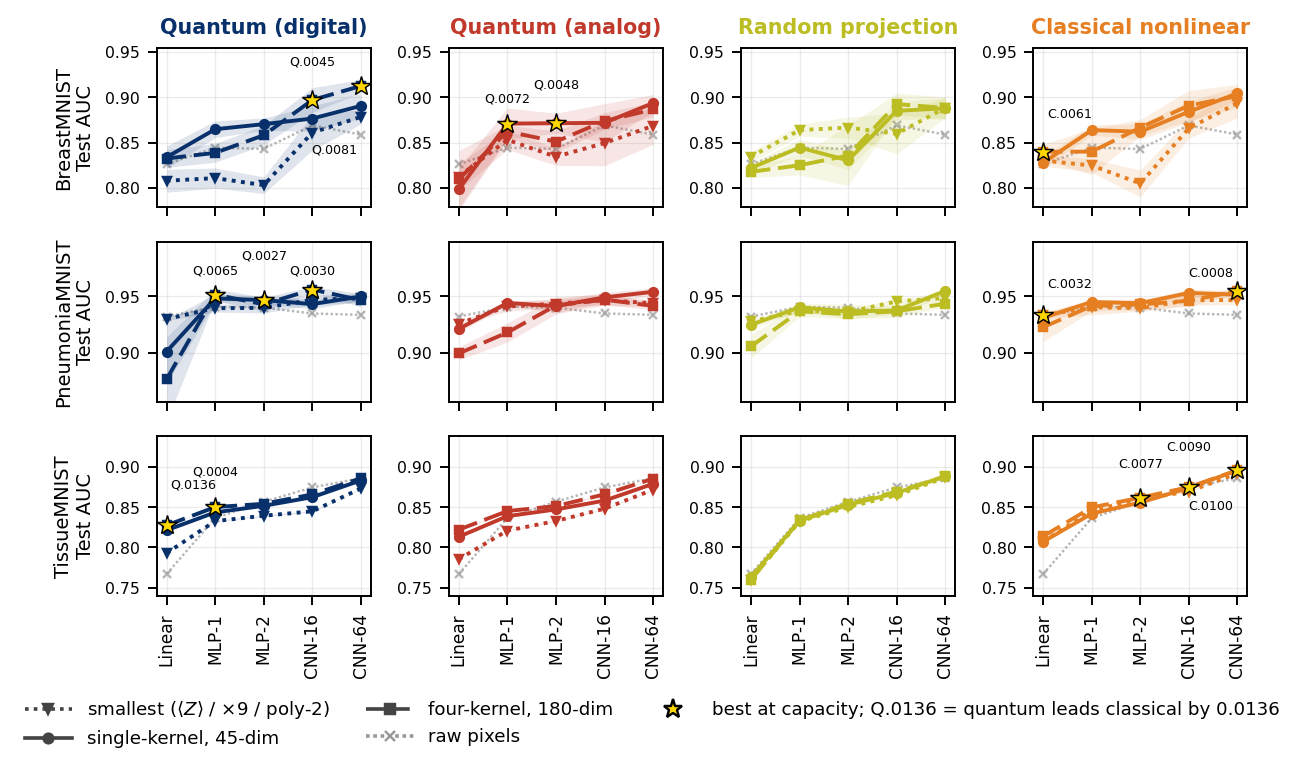
\includegraphics[width=\textwidth]{figures/capacity_sweep_grid.pdf}
\caption{Head-capacity sweep across datasets, on per-feature standardized
inputs. Rows are datasets (BreastMNIST, PneumoniaMNIST, and TissueMNIST);
columns are the four feature families (quantum-digital,
quantum-analog, random projection, classical nonlinear). Each $y$-axis is
shared within its dataset row, and raw pixels are the faint gray anchor in
every panel. Within a panel, scale is encoded by marker and line style:
down-triangle/dotted is the smallest source ($\langle Z\rangle$-only at $9$
features, $\times 9$ random, or poly-2), circle/solid is the single-kernel
$45$-dimensional source, and square/dashed the four-kernel
$180$-dimensional source. Each line is a $10$-seed mean and the shaded
envelope is $\pm 1$ standard deviation across those seeds. At each head a
gold star marks the single best source across all families, labelled by the
winning camp and its margin over the other camp (``Q.0136'' = the best
quantum source leads the best classical source by $0.0136$; ``C'' =
classical leads). The TissueMNIST row uses macro one-vs-rest AUC; its
low-capacity quantum lead survives a
validation-selected topology and bandwidth-and-regularization-tuned
classical baselines (see text), but reverses at the trained-head operating
point (Table~\ref{tab:endtoend}).}
\label{fig:capacity_sweep}
\end{figure*}

The previous two subsections establish that quantum kernels with ZZ
correlators are more linearly separable than dimension-matched random
projections (Section~\ref{sec:results_probing}), yet this advantage
does not propagate cleanly to the end-to-end accuracy table once a
trained CNN head is added (Section~\ref{sec:results_endtoend}).
The head-capacity sweep traces this gap directly as a function of head
expressivity.
As in Section~\ref{sec:method_capacity}, all sources are per-feature
standardized before the head so the comparison reflects information
content rather than feature scale, and the matched-dimension poly-2 and
RFF nonlinear controls test whether any low-capacity advantage is
specific to the quantum kernel or is recovered by classical nonlinearity
alone.

\begin{figure}[t]
\centering
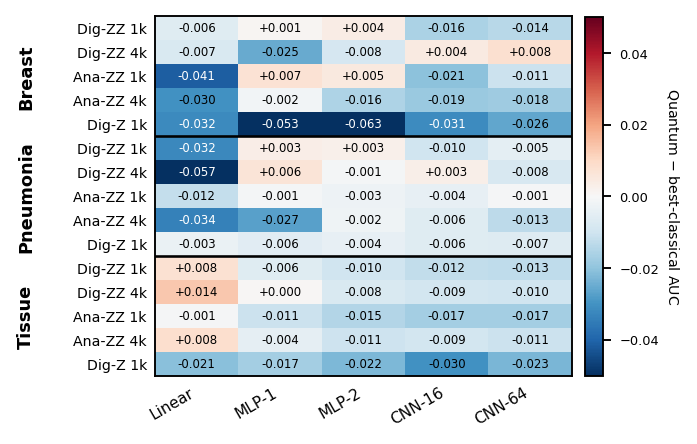
\includegraphics[width=\columnwidth]{figures/capacity_delta_1col.pdf}
\caption{Quantum-minus-classical AUC gap across the capacity ladder. Each cell
is a quantum source's test AUC minus the best classical source at the same
head; red marks the quantum source ahead of every classical source, blue marks
it behind the best classical one. The only positive entries at the linear head
are the four-kernel and single-kernel ZZ cells on TissueMNIST (Digital-ZZ
$+0.014$ and $+0.008$, Analog-ZZ $+0.008$), the verified low-capacity exception;
on the binary datasets the gap is already non-positive and moves toward zero or
negative as the head grows to a trained CNN.}
\label{fig:capacity_delta}
\end{figure}

\subsubsection{Quantum versus classical nonlinearity}
With features standardized, the strongest quantum and strongest
dimension-matched classical sources track each other across the ladder: the
best-quantum minus best-classical AUC stays within $\pm 0.01$ at every head
on both datasets, inside one standard deviation
(Fig.~\ref{fig:capacity_delta}).
The decisive control is the nonlinear map.
Digital-ZZ exceeds the best RFF by at most $+0.008$ AUC at any head,
and on PneumoniaMNIST RFF outperforms it at the linear probe ($-0.030$) and at
CNN-$16$ ($-0.010$).
A matched-dimension classical nonlinear map, the degree-two polynomial or an RBF
random-feature map, thus reproduces whatever the quantum kernel provides.

\subsubsection{Quantum versus random projection, and capacity conditioning}
Against the \emph{linear} random projection the quantum sources do lead at
intermediate capacity ($+0.020$ and $+0.040$ on BreastMNIST at MLP-$1$ and
MLP-$2$, $+0.008$ and $+0.010$ on PneumoniaMNIST, each above one standard
deviation), but RFF achieves a comparable margin, so this lead reflects
nonlinear feature expansion rather than quantum structure, and it converges to
noise at the CNN heads.
The effect is dataset dependent: on the near-separable PneumoniaMNIST the ZZ
quantum sources are the \emph{weakest} at the linear probe, below raw pixels and
most random projections, as the entangling correlators disrupt already-accessible
structure, while the correlator-free Digital-Z stays near the top; only on the
lower-separability BreastMNIST do the quantum sources lead at the probe.

\subsubsection{ZZ ablation across capacities}
The correlator benefit is task dependent.
On BreastMNIST the Digital-ZZ minus Digital-Z gap is large at low capacity
(up to $+0.067$ at MLP-$2$) and positive but within noise at the CNN heads;
on PneumoniaMNIST it is negative at the probe and small thereafter, consistent
with that task being already separable from $\langle Z\rangle$ alone.

\subsubsection{TissueMNIST: a low-capacity exception}
The larger eight-class TissueMNIST is the one task in our study where the
quantum kernel \emph{exceeds} matched classical nonlinearity at low
capacity rather than tying it.
At the linear head of the standardized capacity sweep, Digital-ZZ reaches
macro one-vs-rest AUC $0.828$ at four-kernel scale and $0.822$ at
single-kernel scale, above the best dimension-matched classical nonlinear
map (RFF$\times 180$ $0.814$; RFF$\times 45$ and poly-2 $0.807$), a
$+0.014$ margin that is large relative to the across-seed
spread on this dataset.
The edge survives the fairness controls that dissolved the apparent
BreastMNIST advantage: with the topology selected on a held-out validation
split rather than on test, and the RFF bandwidth and regularization tuned
on validation, a linear probe at matched dimension still favours the
quantum kernel ($+0.005$ over poly-2 and $+0.013$ over the tuned
RFF at $45$ dimensions, $+0.010$ over RFF$\times 180$).
It is nonetheless capacity-limited in the same way as the binary datasets:
an expressive trained head closes and then reverses it, with the best
classical source leading by approximately $0.010$ AUC at the CNN-$64$ head.
The end-to-end operating point (Table~\ref{tab:endtoend},
Section~\ref{sec:results_endtoend}) confirms the reversal: poly-2 leads the
best quantum model by $+0.016$ AUC and even raw pixels exceed every quantum
model, with four-kernel features adding nothing over a single kernel in either
camp.
TissueMNIST therefore sharpens rather than overturns the central finding:
only on the hardest, highest-dimensional task does the quantum kernel beat
\emph{tuned} classical nonlinearity, and only while the head is weak.


\section{Discussion}
\label{sec:discussion}

We draw out four implications of these results, from the role of the ZZ
correlators to where neutral-atom kernels are most likely to help.

\subsection{The ZZ correlators contribute, but only when the task needs them}
On BreastMNIST, single-qubit $\langle Z_i\rangle$ features alone are no more
separable than unstructured random projections, and the pairwise
$\langle Z_iZ_j\rangle$ correlators supply the bulk of the feature map's value;
on the already-separable PneumoniaMNIST the same correlators add essentially
nothing.
The entanglement-mediated correlators help only when the single-qubit
representation is not already linearly separable.

\subsection{The advantage is conditional on classifier capacity and is not
specifically quantum}
The quantum kernels lead a dimension-matched \emph{linear} random projection at
intermediate capacity, but a matched-dimension classical nonlinear feature map
(random Fourier features, and a degree-two polynomial on TissueMNIST)
reproduces that lead, and it shrinks to a tie as capacity grows to a trained CNN
(Fig.~\ref{fig:capacity_sweep});
on the near-separable PneumoniaMNIST the ZZ quantum sources are in fact the
weakest at the linear probe.
The DAQCNN advantage in this regime therefore lives at the feature substrate, is
reproduced by classical nonlinearity, and is absorbed by a sufficiently
expressive trained head.
Because a classical random Fourier map of equal dimensionality reproduces this
advantage on the two binary datasets and is beaten by the quantum kernel only at
low capacity on TissueMNIST, the value of a Rydberg kernel cannot rest on
nonlinearity alone: the narrower defensible case is that the dynamics define a specific
feature-map family that becomes classically intractable to evaluate at large
atom counts, which would require both that hardness and a task aligned with that
family~\cite{liu2021rigorous}, neither of which holds at the nine-qubit scale
tested here.
This matches independent large-scale neutral-atom evidence, where an analog
quantum-reservoir advantage over classical learners appears only on synthetic
datasets built to exhibit a quantum-classical kernel separation, not on natural
data~\cite{kornjaca2024largescale}.

\subsection{When are quantum kernels promising?}
These results suggest that quantum kernels are not universally useful: their
value depends on the alignment between the quantum feature space and the
structure of the data.
The one low-capacity quantum edge we find, on TissueMNIST
(Fig.~\ref{fig:capacity_sweep}, bottom row, linear head), appears precisely
where the single-qubit representation leaves room and the trained head is still
too weak to recover that structure on its own.
We speculate, though our image-only design cannot confirm it, that
graph-structured data is a more natural fit for neutral-atom kernels: their
native interactions and reconfigurable register geometry embed graph structure
directly in the Hamiltonian~\cite{dalyac2024graph}, and neutral-atom quantum
kernels have classified molecular graphs competitively with strong classical
kernels, including on a 32-qubit
processor~\cite{henry2021quantum,albrecht2023graph}, with local detuning further
raising kernel expressiveness~\cite{djellabi2025attributed}.
Our per-patch construction can in fact be read as a single fixed quantum
message-passing step over the nine-pixel patch graph set by the atom-array
topology, applied convolutionally across the image; on graph-native data, where
the topology is the data rather than an imposed prior, the same operator would
act on exactly the structure it encodes.
Domains organised around relational rather than spatial-texture structure, such
as graph learning, physical-system modelling, and scientific relational data, are
therefore a natural target for future work.
We caution, however, that a genuine advantage there remains to be established
under the controls we apply here: existing neutral-atom graph studies benchmark
only against classical graph kernels with a single tuned SVM, not against graph
neural networks or a classifier-capacity sweep, and report competitiveness rather
than a robust win~\cite{henry2021quantum,albrecht2023graph,djellabi2025attributed},
so the same capacity-conditioning and nonlinearity caveats may well apply.
Even a negative result there would be informative, since graphs are the setting
where the platform's inductive bias is most native and thus the cleanest test of
whether a classically-hard, task-aligned kernel advantage exists at all; a frozen
quantum aggregator additionally avoids the barren-plateau trainability problems
that beset variational quantum models~\cite{mcclean2018barren}.

\subsection{Limitations and future work}
Analog encoding's qualitatively broader function class did not translate into a
measurable classification advantage on any of the three datasets, consistent
with image targets dominated by spatial texture; higher-resolution benchmarks
with lower single-qubit separability are a more natural test of an analog edge.
Our kernels are frozen at a single evolution time ($T = 2.5$) and fixed
geometries, so a joint sweep of evolution time and array geometry under both
encodings, paired with measures of generated entanglement and kernel-target
alignment, is the natural next step and a prerequisite for trainable Rydberg
kernels.
Whether the capacity-conditioning verdict persists under a global self-attention
head, whose non-local inductive bias differs from the locality priors of our
linear, MLP, and convolutional ladder, is likewise left to future work.

\section{Conclusion}
\label{sec:conclusion}

We tested whether the quantum-kernel advantage reported for Rydberg-atom DAQCNNs
reflects quantum structure or is an artifact of classifier capacity and feature
nonlinearity.
Across BreastMNIST, PneumoniaMNIST, and the eight-class TissueMNIST, evaluated
with independent per-model hyperparameter searches, multi-seed validation,
dimension-matched classical baselines, and a controlled head-capacity sweep, the
advantage is conditional on the trained classifier: the quantum kernels lead
only a linear random projection at low capacity, are matched by classical
nonlinear feature maps of equal dimensionality, and tie under a trained CNN on
both binary tasks.
The ZZ correlators help only where single-qubit features are not already
separable, and digital and analog encodings perform comparably throughout.
TissueMNIST is the single low-capacity exception, where the quantum kernel
exceeds tuned classical nonlinearity, but a trained head still reverses it.
In this regime the DAQCNN advantage is therefore attributable to nonlinear
feature expansion rather than to quantum structure.


% Acknowledgment omitted in the anonymous submission; add funding and thanks
% for the camera-ready version.

\bibliographystyle{IEEEtran}
\bibliography{references}

\end{document}
